\documentclass{article}

\usepackage{fancyhdr}
\usepackage{extramarks}
\usepackage{amsmath}
\usepackage{amsthm}
\usepackage{amsfonts}
\usepackage{empheq}
\usepackage{mathtools}
\usepackage{physics}
\usepackage{hyperref}
\usepackage[dvipsnames]{xcolor} 
\hypersetup{
	colorlinks,
	linkcolor=BrickRed,
}
\usepackage{tikz}
\usetikzlibrary {datavisualization.formats.functions}
\usepackage{graphicx}
\usepackage{subcaption}
\usepackage{neuralnetwork}
\usepackage{comment}
\usepackage{listings}
\usepackage{matlab-prettifier}
\usepackage{verbatim}
\usepackage[framemethod=tikz]{mdframed}


\newcommand\numberthis{\addtocounter{equation}{1}\tag{\theequation}}

%
% Basic Document Settings
%

\topmargin=-0.45in
\evensidemargin=0in
\oddsidemargin=0in
\textwidth=6.5in
\textheight=9.0in
\headsep=0.25in

\linespread{1.2}

\pagestyle{fancy}
\lhead{\hmwkAuthorName}
\chead{\hmwkClass: \hmwkTitle}
\rhead{\firstxmark}
\lfoot{\lastxmark}
\cfoot{\thepage}

\renewcommand\headrulewidth{0.4pt}
\renewcommand\footrulewidth{0.4pt}

\setlength\parindent{0pt}

%
% Create Question Sections
%

\newcommand{\enterQuestionHeader}[1]{
	\nobreak\extramarks{}{Question \arabic{#1} cont'd on next page\ldots}\nobreak{}
	\nobreak\extramarks{Question \arabic{#1} (cont'd)}{Question \arabic{#1} cont'd on next page\ldots}\nobreak{}
}

\newcommand{\exitQuestionHeader}[1]{
	\nobreak\extramarks{Question \arabic{#1} (cont'd)}{Question \arabic{#1} cont'd on next page\ldots}\nobreak{}
	\stepcounter{#1}
	\nobreak\extramarks{Question \arabic{#1}}{}\nobreak{}
}

\setcounter{secnumdepth}{0}
\newcounter{partCounter}
\newcounter{homeworkQuestionCounter}
\setcounter{homeworkQuestionCounter}{1}
\nobreak\extramarks{Question \arabic{homeworkQuestionCounter}}{}\nobreak{}

%
% Homework Question Environment
%
% This environment takes an optional argument. When given, it will adjust the
% problem counter. This is useful for when the problems given for your
% assignment aren't sequential. See the last 3 problems of this template for an
% example.
%
\newenvironment{homeworkQuestion}[1][-1]{
	\ifnum#1>0
	\setcounter{homeworkQuestionCounter}{#1}
	\fi
	\section{Question \arabic{homeworkQuestionCounter}}
	\rule{0.9\textwidth}{3pt}\\
	\setcounter{partCounter}{1}
	\enterQuestionHeader{homeworkQuestionCounter}
}{
	\exitQuestionHeader{homeworkQuestionCounter}
}

%
% Homework Details
%   - Title
%   - Due date
%   - Class
%   - Section/Time
%   - Instructor
%   - Author
%

\newcommand{\hmwkTitle}{HW\#7}
\newcommand{\hmwkDueDate}{}
\newcommand{\hmwkClass}{CpE 520}
\newcommand{\institute}{West Virginia University}
\newcommand{\hmwkClassInstructor}{Professor Nasser Nasrabadi}
\newcommand{\hmwkAuthorName}{\textbf{Ali Zafari}}

%
% Title Page
%

\title{
	\vspace{2in}
	\textmd{\textbf{\hmwkClass:\ \hmwkTitle}}\\
	\vspace{0.1in}\large{\institute}\\
%	\vspace{0.1in}\large{\textit{\hmwkClassInstructor}}
	\vspace{3in}
}

\author{\hmwkAuthorName}
\date{}

\renewcommand{\part}[1]{\textbf{\Large Part \Alph{partCounter}}\stepcounter{partCounter}\\}



% environment styles for MATLAB code and output
\mdfdefinestyle{matlabcode}{%
	outerlinewidth=.5pt,
	linecolor=gray!20!white,
	roundcorner=2pt,
	innertopmargin=.5\baselineskip,
	innerbottommargin=.5\baselineskip,
	innerleftmargin=2.2em,
	innerrightmargin=0em,
	backgroundcolor=gray!10!white
}


%\newenvironment{matlabcode}{\verbatim}{\endverbatim}

\lstnewenvironment{matlabcode}{\lstset{style=Matlab-editor, numbers=left}}{}
\surroundwithmdframed[style=matlabcode]{matlabcode}

\newenvironment{matlaboutput}{%
	\Verbatim[xleftmargin=1.25em, formatcom=\color{output}]%
}{\endVerbatim}



\begin{document}
	
	\pagenumbering{gobble}% prevent cover page of numbering
	\maketitle
	\pagebreak % let cover page free to the end of page
	\pagenumbering{arabic} % start page numbering again from 1 and print them!
	\tableofcontents
	\pagebreak
	
	\begin{homeworkQuestion}
		
		\subsection{Part (a): Neural Network without Hidden Layer}
		In this part of the question, we are going to train and examine a neural network with no hidden layer (i.e Perceptron). The structure of this network is repeated in figure \ref{fig:q1_parity_1}.
		\begin{figure}[h]
			\centering
			\begin{neuralnetwork}[height=8, nodespacing=1.5cm, layerspacing=6cm, nodesize=40pt]
				\newcommand{\nodetextclear}[2]{}
				\newcommand{\nodetextxnb}[2]{\ifnum #2=4 $\mathbf{X_1X_2}$ \else\ifnum #2=5 $\mathbf{X_1X_3}$ \else\ifnum #2=6 $\mathbf{X_2X_3}$ \else\ifnum #2=7 $\mathbf{X_1X_2X_3}$ \else $\mathbf{X_#2}$ \fi\fi\fi\fi}
				\newcommand{\logiclabel}[1]{\,{$\scriptstyle w_{#1}$}\,}
				\newcommand{\nodetextY}[2]{$\mathbf{y}$}
				\newcommand{\linklabelsA}[4]{\logiclabel{#2} }
				\inputlayer[count=7, bias=true, text=\nodetextxnb]
				\outputlayer[count=7, exclude={1, 2, 3, 5, 6, 7}, text=\nodetextY]
				\link[from layer=0, to layer=1, from node=0, to node=4, label=\linklabelsA]
				\link[from layer=0, to layer=1, from node=1, to node=4, label=\linklabelsA]
				\link[from layer=0, to layer=1, from node=2, to node=4, label=\linklabelsA]
				\link[from layer=0, to layer=1, from node=3, to node=4, label=\linklabelsA]
				\link[from layer=0, to layer=1, from node=4, to node=4, label=\linklabelsA]
				\link[from layer=0, to layer=1, from node=5, to node=4, label=\linklabelsA]
				\link[from layer=0, to layer=1, from node=6, to node=4, label=\linklabelsA]
				\link[from layer=0, to layer=1, from node=7, to node=4, label=\linklabelsA]
			\end{neuralnetwork}
			\caption{Neural network for binary Parity-3}
			\label{fig:q1_parity_1}
		\end{figure}
	
The whole \emph{Matlab} code for training and examining this neural network is printed in the section below:
\begin{matlabcode}[h]
clc
clear variables
close all

% every sample of input lies on a column vector of X
X = zeros(7, 8);
x1 = [0 1];
x2 = [0 1];
x3 = [0 1];

% Input sample generation
for i = 1:size(x1, 2)
	for j = 1:size(x2, 2)
		for k = 1:size(x3, 2)
			X(:, k+2*(j-1)+4*(i-1)) = [x1(i), x2(j), x3(k),...
			x1(i)*x2(j), x1(i)*x3(k),...
			x2(j)*x3(k), x1(i)*x2(j)*x3(k)];
		end
	end
end

t = [0 1 1 0 1 0 0 1];

% the initialization which converges
rng(3);
net = patternnet([]);
net.divideFcn = 'dividetrain';
net.performFcn = 'mse';
net.trainParam.showCommandLine = 1;
net.trainParam.show = 1;

[net, tr, y, e] = train(net, X, t);

weights_in = net.IW;
weights_hidden = net.LW;
biases  = net.b;
view(net);
\end{matlabcode}


The resulting \emph{Matlab}-generated block diagram of the neural network is shown in figure \ref{fig:block_diagram_1}.
\begin{figure}[h]
	\centering
	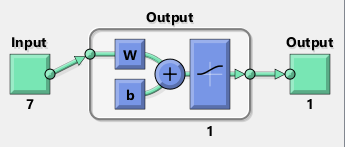
\includegraphics[width=0.6\linewidth]{HW7_1_block_diagram}
	\caption{ \emph{Matlab}-generated block diagram}
	\label{fig:block_diagram_1}
\end{figure}

\clearpage
Learning curve which shows the decreasing value of mean square error versus the number of epochs is plotted in figure \ref{fig:error_1}. It shows that after 74 epochs the network is trained successfully.
\begin{figure}[h]
	\centering
	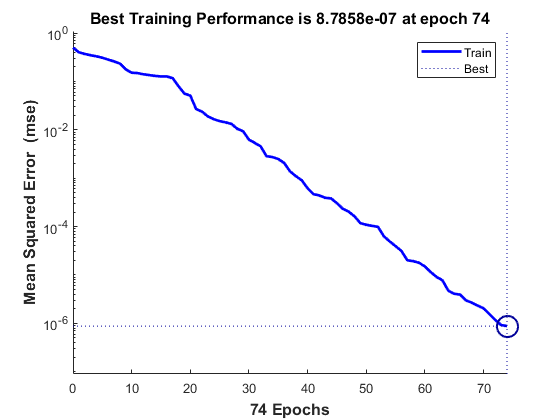
\includegraphics[width=0.9\linewidth]{HW7_1}
	\caption{MSE versus epoch number}
	\label{fig:error_1}
\end{figure}

Calculated weights of the whole network are reported in table \ref{tab:weights_1}.
\begin{table}[h]
	\centering 
	\caption{Weights of the neural network}
	\begin{tabular}{c|c|c|c|c|c|c|c} 
		\hline 
		$w_{0}$&$w_{1}$&$w_{2}$&$w_{3}$&$w_{4}$&$w_{5}$&$w_{6}$&$w_{7}$\\ [0.5ex] 
		\hline\hline
		$0.94$&$6.78$&$6.71$&$6.78$&$-13.75$&$-13.74$&$-13.73$&$28.54$\\[1ex]
		\hline
	\end{tabular}
	\label{tab:weights_1}
\end{table}

\clearpage


\subsection{Part (b): Neural Network with Hidden Layer}
		Unlike the neural network of previous part, the structure of network in this part includes a fully connected hidden layer as it is shown in figure \ref{fig:q1_parity_2}. 
		\begin{figure}[h]
			\centering
			\begin{neuralnetwork}[height=5, nodespacing=2cm, layerspacing=5cm, nodesize=20pt]
				\newcommand{\nodetextclear}[2]{}
				\newcommand{\nodetextxnb}[2]{$\mathbf{X_#2}$}
				\newcommand{\nodetextH}[2]{$\mathbf{h_#2}$}
				\newcommand{\nodetextY}[2]{$\mathbf{y}$}
				\newcommand{\logiclabels}[3]{\,$\scriptstyle w_{#1#2}^#3$\,}
				\newcommand{\linklabelsX}[4]{\logiclabels{#2}{#4}{#1}}
				\newcommand{\linklabelsy}[4]{\logiclabels{#2}{}{#1}}
				\inputlayer[count=3, bias=true, text=\nodetextxnb]
				\hiddenlayer[count=3, bias=true, text=\nodetextH]
				\outputlayer[count=4, exclude={1, 2, 4}, text=\nodetextY]
				\link[from layer=0, to layer=1, from node=0, to node=1, label=\linklabelsX, labelpos=very near start]
				\link[from layer=0, to layer=1, from node=0, to node=2, label=\linklabelsX, labelpos=very near start]
				\link[from layer=0, to layer=1, from node=0, to node=3, label=\linklabelsX, labelpos=very near start]
				\link[from layer=0, to layer=1, from node=1, to node=1, label=\linklabelsX, labelpos=very near start]
				\link[from layer=0, to layer=1, from node=1, to node=2, label=\linklabelsX, labelpos=very near start]
				\link[from layer=0, to layer=1, from node=1, to node=3, label=\linklabelsX, labelpos=very near start]
				\link[from layer=0, to layer=1, from node=2, to node=1, label=\linklabelsX, labelpos=very near start]
				\link[from layer=0, to layer=1, from node=2, to node=2, label=\linklabelsX, labelpos=very near start]
				\link[from layer=0, to layer=1, from node=2, to node=3, label=\linklabelsX, labelpos=very near start]
				\link[from layer=0, to layer=1, from node=3, to node=1, label=\linklabelsX, labelpos=very near start]
				\link[from layer=0, to layer=1, from node=3, to node=2, label=\linklabelsX, labelpos=very near start]
				\link[from layer=0, to layer=1, from node=3, to node=3, label=\linklabelsX, labelpos=very near start]
				\link[from layer=1, to layer=2, from node=0, to node=3, label=\linklabelsy]
				\link[from layer=1, to layer=2, from node=1, to node=3, label=\linklabelsy]
				\link[from layer=1, to layer=2, from node=2, to node=3, label=\linklabelsy]
				\link[from layer=1, to layer=2, from node=3, to node=3, label=\linklabelsy]
			\end{neuralnetwork}
			\caption{Neural network for binary Parity-3}
			\label{fig:q1_parity_2}
		\end{figure}
	
	The whole \emph{Matlab} code for training and examining this neural network is printed in the section below:
	\begin{matlabcode}[h]
clc
clear variables
close all

% every sample of input lies on a column vector of X
X = zeros(3, 8);
x1 = [0 1];
x2 = [0 1];
x3 = [0 1];

% Input sample generation
for i = 1:size(x1, 2)
	for j = 1:size(x2, 2)
		for k = 1:size(x3, 2)
			X(:, k+2*(j-1)+4*(i-1)) = [x1(i), x2(j), x3(k)];
		end
	end
end

%target outputs
t = [0 1 1 0 1 0 0 1];

% the initialization which converges
rng(10);
net = patternnet(3);
net.divideFcn = 'dividetrain';
net.performFcn = 'mse';
net.trainParam.showCommandLine = 1;
net.trainParam.show = 1;

[net, tr, y, e] = train(net, X, t);

weights_in = net.IW;
weights_hidden = net.LW;
biases  = net.b;
view(net);
	\end{matlabcode}

The resulting \emph{Matlab}-generated block diagram of the neural network is shown in figure \ref{fig:block_diagram_2}.\\

\begin{figure}[h]
	\centering
	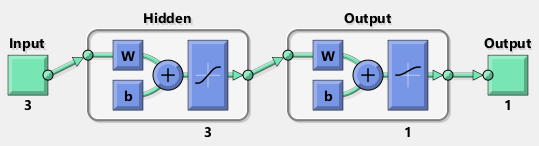
\includegraphics[width=0.7\linewidth]{HW7_2_block_diagram}
	\caption{ \emph{Matlab}-generated block diagram}
	\label{fig:block_diagram_2}
\end{figure}
\clearpage

Learning curve which shows the decreasing value of mean square error versus the number of epochs is plotted in figure \ref{fig:error_2}. It shows that after 94 epochs the network is trained successfully.
\begin{figure}[h]
	\centering
	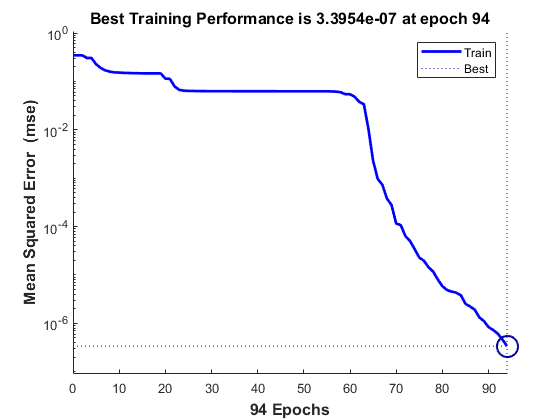
\includegraphics[width=0.7\linewidth]{HW7_2}
	\caption{MSE versus epoch number}
	\label{fig:error_2}
\end{figure}

Calculated weights of the whole network are reported in tables \ref{tab:weights_2_1} and \ref{tab:weights_2_2}.
\begin{table}[h]
	\centering 
	\caption{Weights of the 1st layer of neural network}
		\begin{tabular}[\linewidth]{c|c|c|c|c|c|c|c|c|c|c|c} 
			\hline 
			$w_{01}^0$&$w_{02}^0$&$w_{03}^0$&$w_{11}^0$&$w_{12}^0$&$w_{13}^0$&$w_{21}^0$&$w_{22}^0$&$w_{23}^0$&$w_{31}^0$&$w_{32}^0$&$w_{33}^0$\\ [0.5ex] 
			\hline\hline
			$-0.19$&$-0.80$&$3.49$&$-4.17$&$-3.92$&$-2.97$&$-6.48$&$-6.45$&$3.22$&$-0.02$&$-0.01$&$4.41$\\[1ex] 
			\hline
		\end{tabular}
	\label{tab:weights_2_1}
\end{table}

\begin{table}[h]
	\centering 
	\caption{Weights of the 2nd layer of neural network}
	\begin{tabular}[\linewidth]{c|c|c|c} 
		\hline 
		$w_{0}^1$&$w_{1}^1$&$w_{2}^1$&$w_{2}^1$ \\ [0.5ex] 
		\hline\hline
		$-1.35$&$7.53$&$-7.52$&$8.618$\\[1ex] 
		\hline
	\end{tabular}
	\label{tab:weights_2_2}
\end{table}

	\end{homeworkQuestion}

\end{document}